\documentclass[12pt,a4paper]{article}

\usepackage[utf8]{inputenc}
\usepackage{graphicx}
\usepackage{hyperref}
\usepackage{listings}
\usepackage{float}
\usepackage[margin=2.5cm]{geometry}
\usepackage{subfiles}


\usepackage{natbib} 
\usepackage{graphicx}
\usepackage{xcolor}
\usepackage{amsmath,amssymb,amsfonts,amsthm}
\usepackage{enumitem}
\usepackage{nameref}
\usepackage{booktabs}
%\usepackage{listings}
\usepackage{algorithm,algorithmic}
\usepackage{mathtools}
\usepackage{placeins}
\usepackage{subfiles}
\usepackage{bm}
\usepackage{stfloats}
\usepackage{rotating}
\usepackage{libertine} 
\usepackage{tabularx}
\usepackage{hyperref}
\usepackage{xcolor}
\usepackage{subfiles} % Best loaded last in the preamble



\begin{document}
\subfile{title}

\begin{abstract}
\noindent \small 
This is the Abstract 
\end{abstract}

\small \tableofcontents

\begin{appendix}
  \small \bibliographystyle{plain} % 'ieee', 'acm', 'alpha'
  \small \bibliography{references}
  \small \listoffigures
\end{appendix}

\newpage

\section{Introduction}
This section provides an overview of the project, including the motivation, and the research question.

\subsection{Motivation}

The digital entertainment landscape has transformed, with unprecedented content production and availability.
However, this abundance of choice has become a burden for consumers.
Streaming platforms prioritize user retention
over satisfaction, resulting in suboptimal viewing experiences.
Content discovery is challenging due to cognitive load from navigating extensive catalogs across multiple services.
Existing recommendation systems exhibit biases towards platform-specific content and popular titles, wasting user time.
A user-centric approach is needed, prioritizing user time and preferences over platform metrics.

\subsection{Research Question}

This project addresses a central research question:
How can we build a central system using a transformer-based architecture to process natural language queries,
to generate personalized movie recommendations and efficetly reduce the users effort of finding matching content?
\newline \noindent This question encompasses advanced natural language processing, maintaining recommendation relevance, and system
adaptability through user feedback. It directly addresses creating a more efficient and user-centric content discovery
platform while acknowledging technical complexity in processing user preferences and ensuring system responsiveness.

\section{Related Work}

This section provides an overview of the literature and a brief discussion regarding our project.
This section starts with a brief overview of the literature, followed by a discussion of our actual project implementation.

\subsection{Literature}

There are several approaches to movie recommendation systems.
For the literature overview we focus on literature matching the context of the ``Advanced Information Retrieval'' course.
One paper espcially caught our attention, as it uses a transformer-based architecture to generate movie recommendations,
but also discusses foundtaional steps like data preprocessing and dimensionality reduction.
This is especially of interest to us, as the whole topic is novel to us and we are looking for a good starting point.

\noindent One team of researchers \cite{Iglesias-pardo-lopez-quintero-2024} proposes a movie recommendation system that uses a
transformer-based embeddings space. To achieve this it was necessary to perform dimensionality reduction.
The first thing, as in many data science projects, is to preprocess the data.
In the case of the discussed project the dataset of 45.466 movies was reduced to just 11.236 \cite{Iglesias-pardo-lopez-quintero-2024}.
The features of the movies where transformed to a matrix consisting of id, original title, release date,
original language, runtime, vote average, vote count, popularity, poster path, production companies, genres, overview,
keywords, cast, director and release year \cite{Iglesias-pardo-lopez-quintero-2024}.
To generate meaningful embeddings of sentences the a variation of the BERT-family of models was used \cite{Iglesias-pardo-lopez-quintero-2024}.
Through the usage of dimensionality reduction they were able to visualize the movies on a 2D-plane \cite{Iglesias-pardo-lopez-quintero-2024}.

\noindent The mentioned steps already provide good insight into a starting point for such a system.
This was a good orientation for our project, but the actual user-interaction is highly different than our approach.
In the case of the mentioned project the user is able to select 10 movies and the system will then generate a recommendation \cite{Iglesias-pardo-lopez-quintero-2024}.
Afterwards the user is asked to rate the recommendation and the system will generate a new recommendation based on the feedback \cite{Iglesias-pardo-lopez-quintero-2024}.

\subsection{Project Discussion}

After reviewing the literature, we browsed through \href{https://www.huggingface.com/}{HuggingFace} to find datasets,
models and other resources to build our system.
This was also the most informative part of our own research as we gathered lots of ideas and insights from the community
and through the extensive collection of readmes and whitepapers on the platform.
This sophisticated movie recommendation system uses multiple advanced methods to deliver personalized movie recommendations.
It aims to use a approach balanced between computational efficiency, accuracy, and user experience.
The system evluates recommendations based on five key parts:
\begin{itemize}
  \item Semantic Analysis (40\%): Uses the MPNet-based SentenceTransformer model to capture deep contextual understanding of movie descriptions and user preferences.
  \item TF-IDF Similarity (40\%): Captures specific terminology and phrases.
  \item Emotion Analysis (15\%): Using text-classification as a foundation the emotional accordance with the movie content and the mood choice by the user is evaluated.
  \item Vote Average Metrics (2,5\%): One out of two factors to ensure recommendations remain somewhat connected to mainstream appeal.
  \item Popularity Metrics (2,5\%): One out of two factors to ensure recommendations remain somewhat connected to mainstream appeal.
\end{itemize}

\noindent The system’s robustness is enhanced through efficient text preprocessing, caching, batch processing and GPU (CUDA, MPS) acceleration.

\noindent Recommendation Generation Process:
\begin{itemize}
  \item Filtering dataset based on trivial criteria (e.g. language, genres).
  \item Initial query processing combines user mood preferences with notes.
  \item Multi-stage similarity computation generates semantic embeddings for the query and movie corpus, then calculates TF-IDF similarity, sentiment alignment, and popularity normalization.
  \item Final ranking selects top recommendations based on weighted scores.
\end{itemize}

\noindent To further improve the user experience, we integrated subtitle analysis using the facebook/bart-large-cnn model. 
The subtitles of movies were sourced from OpenSubtitles API\footnote{\label{OpenSubtitles}OpenSubtitles. December 2024. url: https://www.opensubtitles.org}., pre-processed and run through the summary model to create an introductory summary of each movie. 
The summary model only processes the beginning of the subtitles so that it gives users an insight into the movie without spoilers. 
In addition, KeyBERT was used to extract three key themes from the subtitles and present them to the user. 
\newline \\
\noindent This system is well-suited for streaming platform recommendation engines, personalized content curation, movie discovery and educational purposes.
Due to it's modular design (frontend / backend strictly separated) it can be easily integrated into existing systems.
The frontend is optionally deployable as the backend can be integrated into any existing system due to interfacing
using a easy-to-understand REST API.

\section{Experiments and Results}

To evaluate the performance, feasibility, and efficiency of our system, a series of experiments were conducted.
A standardized questionnaire was employed to assess the system’s performance.
Each group member independently evaluated the system.
This evaluation process was iterated over three days to identify a movie for each evening’s viewing.
The individual evaluation reports can be found in the appendix folder within the
\href{https://github.com/IImpaq/air-2024/appendix}{project repository}.
The evaluation results of each group member were averaged to provide a comprehensive overview of the system’s performance.
Our finalized results and evaluation is presented in the following paragraph.

% TODO Add results of subjective evaluation

\noindent The second part of the evaluation was to objectively and quantifiably evaluate the system through a evaluation script.
This script measured different metrics like response time, confidence score and genre distribution.
Aftwards a variety of metrics was calculated to evaluate the system.
The evaluation script also measured statistical metrics like precision, recall and F1-score.
We are going to use the rest of this section to discuss the most relevant metrics and results of the evaluation.
The evaluation script was called with the following parameters:
\begin{itemize}
  \item use randomly sampled 20\% of the full dataset for evaluation
  \item run each test case 2 times and take the average
  \item sample 1000 testcases from all generated tests to evaluate the system
\end{itemize}

\noindent The script was executed on a MacBook Pro 14" with a M3 Pro chip and 18GB of RAM in a Python 3.12.6 environment.
In the following figure we can see the distribution of response times of the recommendation system.

\begin{figure}[H]
  \centering
  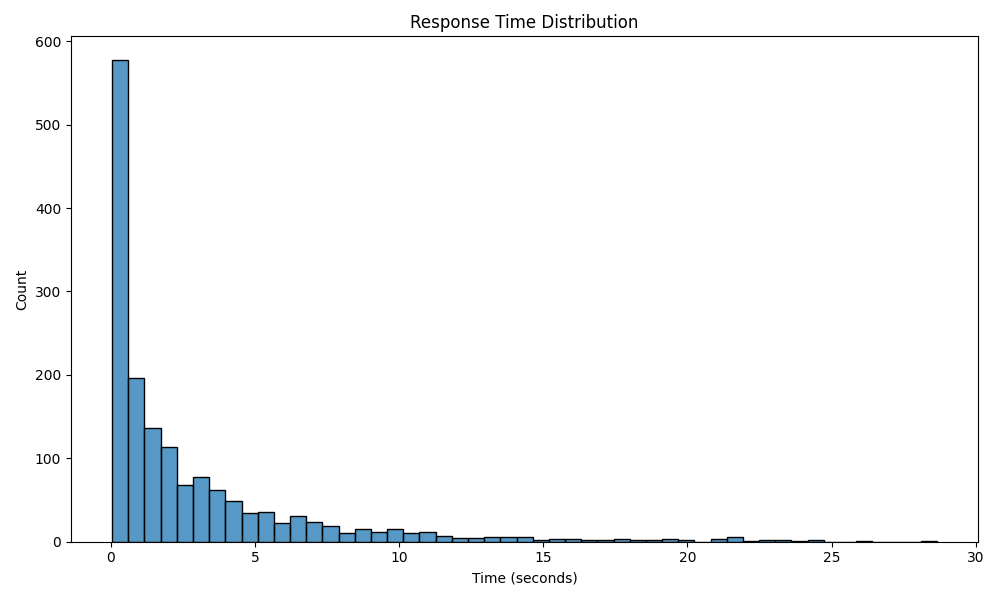
\includegraphics[width=0.4\textwidth]{../assets/response_time_dist.png}
  \caption{Response time}
\end{figure}

\noindent This figure shows that sometimes the system is unable to provide results which causes a nearly instant response.
In a majority of the cases the system is able to provide results within 4 seconds which is reasonable given the complexity of the system and the used hardware.
There are also some outliers which have taken more than 10 seconds to provide results.
In the next figure we can see the distribution of confidence scores of the recommendation system.

\begin{figure}[H]
  \centering
  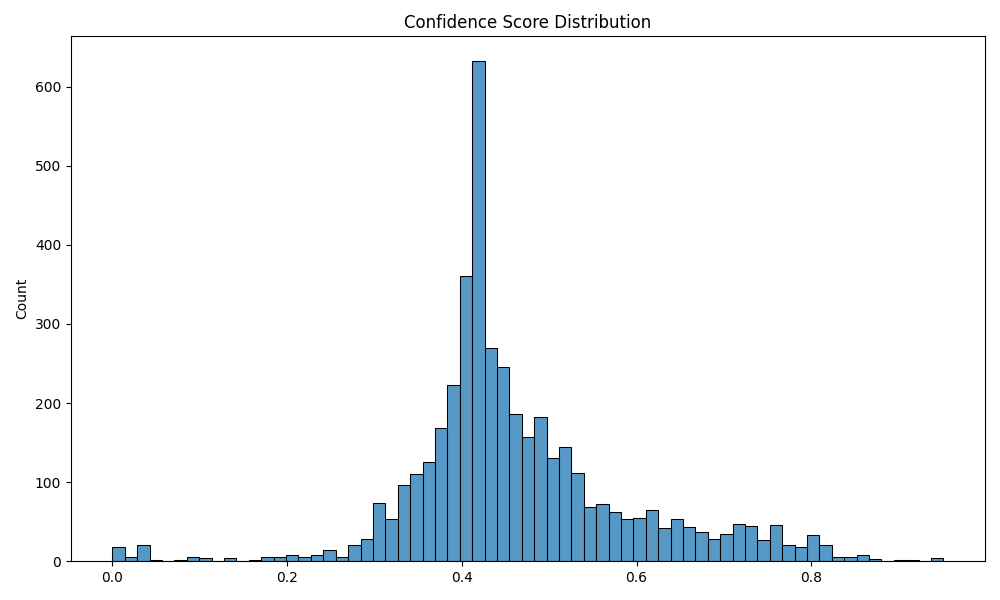
\includegraphics[width=0.4\textwidth]{../assets/confidence_dist.png}
  \caption{Confidence score}
\end{figure}

\noindent The figure shows that the system mostly has a confidence score of 42\% which could be better.
In the last figure we can see the distribution of genre distribution of the recommendation system visualized in a histogram.

\begin{figure}[H]
  \centering
  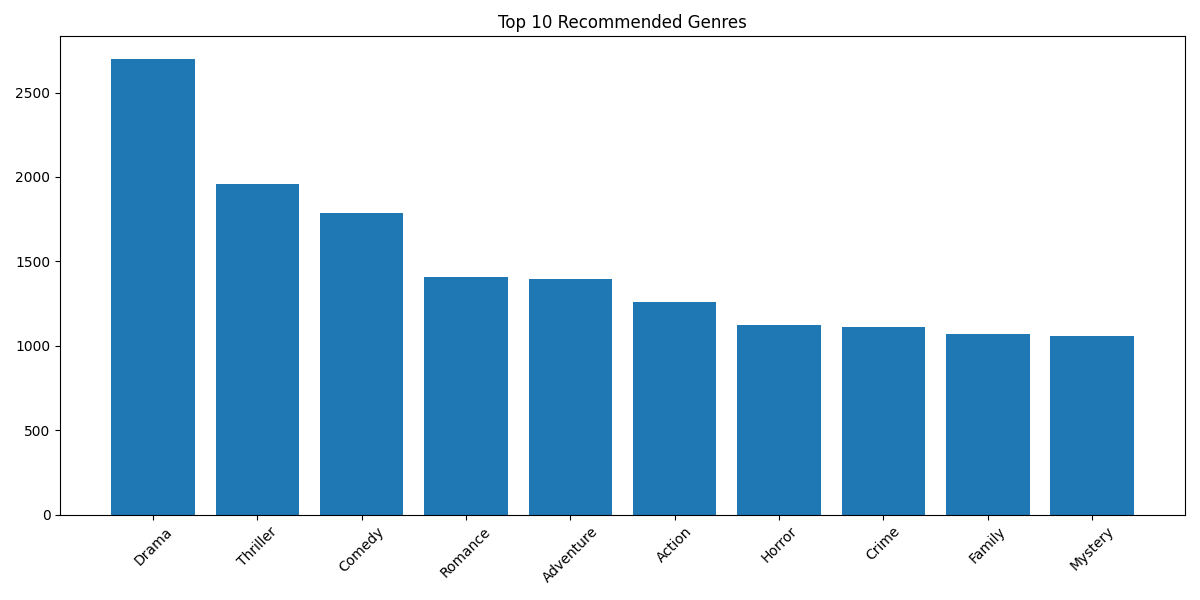
\includegraphics[width=0.4\textwidth]{../assets/top_genres.png}
  \caption{Genre distribution histogram}
\end{figure}

\noindent The figure clearly shows that the system is able to recommend movies from a wide variety of genres.
Some are recommended more often than others, but the system does not show a clear bias towards a specific genre.
\newline \noindent If we take a look at the statistical metrics we can see that the system performs quite well.
The precision of the system is 98.78\% which indicates that the system is very good at recommending movies that the user likes.
The recall of the system is 21.96\% which indicates that the system might be missing out on some movies that the user likes.
The F1-score of the system is 29.17\% which is relatively low, but was expected due to the low recall.

The mentioned values, complete results as well as other plots can be found in the evaluation folder within the \href{https://github.com/IImpaq/air-2024/evaluation}{project repository}.

\section{Conclusion}

In the project we managed to produce highly usable and efficient movie recommendations.
Nonetheless, there is still a lot of tweaking and fine-tuning to be done.
Minor changes can lead to significant improvements in the user experience as we already noticed during development.

\end{document}
